\documentclass[12pt]{article}
\usepackage[margin=2.5cm]{geometry}
\usepackage{enumerate}
\usepackage{amsfonts}
\usepackage{amsmath}
\usepackage{fancyhdr}
\usepackage{amsmath}
\usepackage{amssymb}
\usepackage{amsthm}
\usepackage{mdframed}
\usepackage{graphicx}
\usepackage{subcaption}
\usepackage{adjustbox}
\usepackage{listings}
\usepackage{xcolor}
\usepackage{courier}
\usepackage[utf]{kotex}
\usepackage{hyperref}
\usepackage{soul}
\usepackage{cancel}


\definecolor{codegreen}{rgb}{0,0.6,0}
\definecolor{codegray}{rgb}{0.5,0.5,0.5}
\definecolor{codepurple}{rgb}{0.58,0,0.82}
\definecolor{backcolour}{rgb}{0.95,0.95,0.92}

\lstdefinestyle{mystyle}{
    backgroundcolor=\color{backcolour},
    commentstyle=\color{codegreen},
    keywordstyle=\color{magenta},
    numberstyle=\tiny\color{codegray},
    stringstyle=\color{codepurple},
    basicstyle=\ttfamily\footnotesize,
    breakatwhitespace=false,
    breaklines=true,
    captionpos=b,
    keepspaces=true,
    numbers=left,
    numbersep=5pt,
    showspaces=false,
    showstringspaces=false,
    showtabs=false,
    tabsize=1
}

\lstset{style=mystyle}

\pagestyle{fancy}
\renewcommand{\headrulewidth}{0.4pt}
\lhead{Codeacademy}
\rhead{Notes}

\begin{document}
\title{Codeacademy Notes}

\section{Build a Back-End with Node/Express.js}
\subsection{Introduction}
\subsection{Node REPL}
\begin{itemize}
    \item Is an abbrebivation for Read-eval-print loop
    \item Node comes with built-in javascript REPL
    \item \texttt{.editor} goes into editor mode
    \begin{itemize}
        \item Use \texttt{CTRL + D} when ready to evaluate the input
    \end{itemize}
    \item A REPL can be extremely useful for performing calculations
    \item The Node environment contains a number of Node-specific \texttt{global}
    elements in addition to those built into the JavaScript language
    \begin{itemize}
        \item can be examined using command \texttt{console.log(global)}
    \end{itemize}
\end{itemize}

\subsection{Running a Program with Node}
\begin{itemize}
    \item Done using command \texttt{node myProgram.js}
    \item Javascript code is written to file \texttt{.js} extension
\end{itemize}

\subsection{Accessing the Process Object}
\begin{itemize}
    \item Node has a global \texttt{process} object with useful methods and information about the current process.
    \begin{itemize}
        \item \texttt{process.env} property is an object which stores and controls information about the environment in which the process is currently running
        \begin{itemize}
            \item \texttt{PWD} - holds a string with the directory where the current process is located
            \item \texttt{NODE\_ENV} - holds a value of either production or development

            \bigskip

            \underline{\textbf{Example}}

    \begin{lstlisting}
    if (process.env.NODE_ENV === 'development'){
        console.log('Testing! Testing! Does everything work?');
    }
    \end{lstlisting}

            \item \texttt{process.memoryUsage()} returns information on the CPU demands of the current process.
            \item \texttt{process.memoryUsage().heapUsed} return a number representing how many bytes of memory the current process is using.
        \end{itemize}
        \item \texttt{process.argv} property holds an array of command line values provided when the current process was initiated
        \begin{itemize}
            \item first element in the array is the absolute path to Node
            \item second element in the array is the path to the file that’s running
            \item following elements will be any command line arguments provided when the process was initiated (like C)!!!
        \end{itemize}

    \begin{lstlisting}
    node myProgram.js testing several features
    \end{lstlisting}

    \begin{lstlisting}
    console.log(process.argv[3]); // Prints 'several'
    \end{lstlisting}
    \end{itemize}
\end{itemize}

\subsection{Core Modules and Local Modules}
\begin{itemize}
    \item \textbf{Modularity} is a software design technique where one program has distinct parts each providing a single piece of the overall functionality.
    \begin{itemize}
        \item Is essential when creating scalable programs
        \begin{itemize}
            \item incorporate libraries and frameworks and separate the program’s concerns into manageable chunks
        \end{itemize}
    \end{itemize}
    \item \textbf{Modules} come together to build a cohesive whole
    \begin{itemize}
        \item is imported using \texttt{require()}

    \begin{lstlisting}
    // Require in the 'events' core module:
    let events = require('events');
    \end{lstlisting}

        \item is exported using \texttt{module.exports}

    \begin{lstlisting}
    module.exports = class Dog {

        constructor(name) {
            this.name = name;
        }

        praise() {
            return `Good dog, ${this.name}!`;
        }
    };
    \end{lstlisting}
    \end{itemize}
\end{itemize}

\subsection{Node Package Manager}
\begin{itemize}
    \item NPM, which stands for Node Package Manager
\end{itemize}

\subsection{Event-Driven Architecture}
\begin{itemize}
    \item Node is often described as having event-driven architecture
    \item Node provides an \texttt{EventEmitter} class which we can access by requiring in the events core module
    \begin{lstlisting}
    // Require in the 'events' core module
    let events = require('events');

    // Create an instance of the EventEmitter class
    let myEmitter = new events.EventEmitter();
    \end{lstlisting}
\end{itemize}

\subsection{Event-Driven Architecture}
\begin{itemize}
    \item Node is often described as having event-driven architecture.
    \begin{itemize}
        \item This feels so much like threaded programming
    \end{itemize}
    \item event emitter instance has an \texttt{.on()} method which assigns a listener callback function to a named event.
    \begin{itemize}
        \item first argument - the name of the event as a string
        \item second argument - the listener callback function
    \end{itemize}

    \begin{lstlisting}

    let newUserListener = (data) => {
        console.log(`We have a new user: ${data}.`);
    };

    // Assign the newUserListener function as the listener callback for 'new user' events
    myEmitter.on('new user', newUserListener)

    // Emit a 'new user' event
    myEmitter.emit('new user', 'Lily Pad') //newUserListener will be invoked with 'Lily Pad'
    \end{lstlisting}
\end{itemize}

\subsection{Asynchronous JavaScript with Node.js}
\begin{itemize}
    \item Node was designed to use an event loop like the one used in browser-based JavaScript execution
    \item The event-loop enables asynchronous actions to be handled in a non-blocking way.
    \begin{itemize}
        \item APIs trigger the subscription to and \ul{emitting of events to signal the completion of the operation}
    \end{itemize}

    \underline{\textbf{Example}}

    \bigskip

    \begin{lstlisting}
    let keepGoing = true;

    let callback = () => {
        keepGoing = false;
    };

    setTimeout(callback, 1000); // Run callback after 1000ms

    while(keepGoing === true) {
        console.log(`This is the song that never ends. Yes, it just goes on and on my friends. Some people started singing it, not knowing what it was, and they'll continue singing it forever just because...`)
    };
    \end{lstlisting}

    \begin{itemize}
        \item The while loop will continue forever
        \item Why? because no signal has been sent
        \item To resolve this issue, replace \texttt{setTimeout} with \texttt{setTimeInterval}
    \end{itemize}
    \item \texttt{Promise}, \texttt{async ... await}
    \begin{itemize}
        \item modern way of handling asynchronous tasks
    \end{itemize}
\end{itemize}

\subsection{Asynchronous Javascript - Introduction}
\begin{itemize}
    \item \textbf{asynchronous operation} is one that allows the computer to “move on” to other tasks while waiting for the asynchronous operation to complete.
\end{itemize}

\subsection{Asynchronous Javascript - What is a Promise?}

\begin{center}
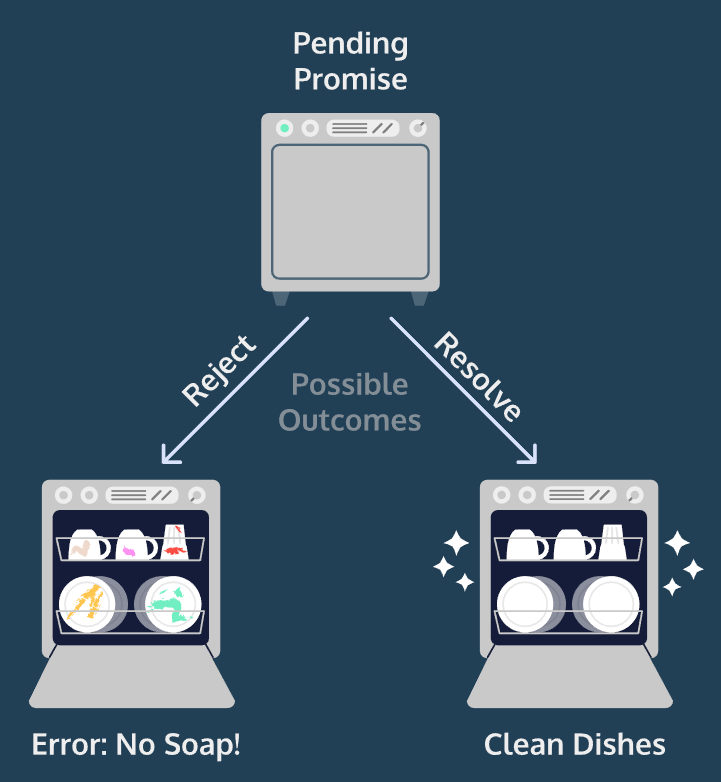
\includegraphics[width=0.9\linewidth]{images/tutorial_2.png}
\end{center}

\begin{itemize}
    \item \textbf{Pending:} The initial state— the operation has not completed yet.
    \item \textbf{Fulfilled:} The initial state— the operation has not completed yet.
    \item \textbf{Rejected:} The initial state— the operation has not completed yet.
\end{itemize}

\subsection{Constructing a Promise Object}
\begin{itemize}
    \item use the \texttt{new} keyword and the \texttt{Promise} constructor method

    \begin{lstlisting}
    const executorFunction = (resolve, reject) => { };
    const myFirstPromise = new Promise(executorFunction);
    \end{lstlisting}

    \item \texttt{Promise} constructor method takes a function parameter called the
    \texttt{executor} function which runs automatically when the constructor is called

    \item The \texttt{executor} function has has two function parameters
    \begin{itemize}
        \item \texttt{resolve()}
        \begin{itemize}
            \item is a function with one arguement
            \item invoke causes the promise's status to change from \texttt{pending} to \texttt{fulfilled}
            \item sets promises' resolved value to be the arguement passed to \texttt{resolve}
        \end{itemize}
        \item \texttt{reject()}
        \begin{itemize}
            \item takes a reason or error as an argument
            \item invoke causes \texttt{reject()} to change the promise’s status from \texttt{pending} to \texttt{rejected}
        \end{itemize}
    \end{itemize}

    \bigskip

    \underline{\textbf{Example}}

    \begin{lstlisting}
    const executorFunction = (resolve, reject) => {
        if (someCondition) {
            resolve('I resolved!');
        } else {
            reject('I rejected!');
        }
    }
    const myFirstPromise = new Promise(executorFunction);
    \end{lstlisting}

\end{itemize}

\subsection{The Node setTimeout() Function}

\begin{center}
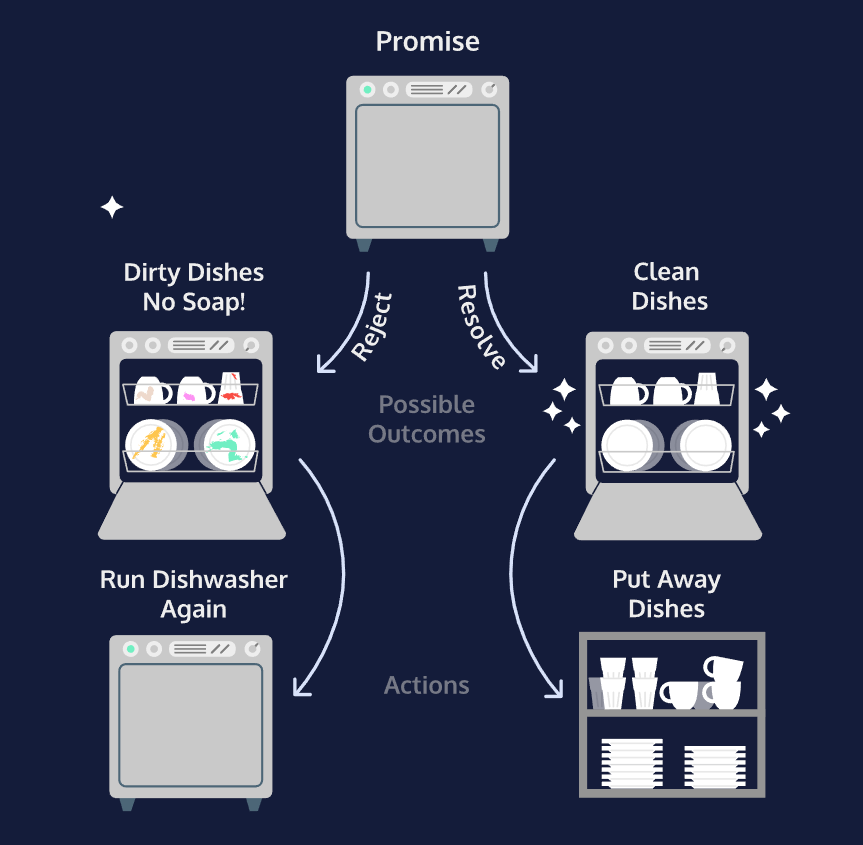
\includegraphics[width=0.9\linewidth]{images/tutorial_3.png}
\end{center}


\begin{itemize}

    \item Rather than constructing promises, you’ll be handling \texttt{Promise} objects returned to you as the result of an asynchronous operation
    \begin{itemize}
        \item It will start off pending but settle eventually.
    \end{itemize}

    \item \texttt{setTimeout()}
    \begin{itemize}
        \item Is a node API
        \item Has two parameters
        \begin{itemize}
            \item a callback function
            \item a delay in milliseconds.
        \end{itemize}

        \begin{lstlisting}
        const executorFunction = (resolve, reject) => {
            if (someCondition) {
                resolve('I resolved!');
            } else {
                reject('I rejected!');
            }
        }
        const myFirstPromise = new Promise(executorFunction);
        \end{lstlisting}

    \end{itemize}

    \item the embedded code will exectue after said time (not exactly at the time)
    \begin{itemize}
        \item because the function within is added to a line of code waiting to be run
    \end{itemize}
\end{itemize}

\subsection{Consuming Promises}
\begin{itemize}
    \item \texttt{.then()} is that it always returns a promise. We’ll return to this in more detail in a later exercise and explore why it’s so important.
    \item \texttt{.then()} takes two callback functions as arguements
    \begin{itemize}
        \item First argument - is the success handler
        \item Second argument - is the failure handler
    \end{itemize}
\end{itemize}

\subsection{The onFulfilled and onRejected Functions}

\subsection{Using catch() with Promises}
\begin{itemize}
    \item \texttt{separation of concerns} - one way to write cleaner code
    \item Javascript doesn't mind whitespace
    \item \texttt{.catch()} function takes only one argument, onRejected

    \bigskip

    \underline{\textbf{Example}}

    \begin{lstlisting}
    prom
    .then((resolvedValue) => {
        console.log(resolvedValue);
    })
    .catch((rejectionReason) => {
        console.log(rejectionReason);
    });
    \end{lstlisting}

\end{itemize}

\subsection{Chaining Multiple Promises}
\begin{itemize}
    \item \texttt{composition} - the process of chaining promises together
    \item Promise is designed with composition in mind

    \bigskip

    \underline{\textbf{Example}}

    \begin{lstlisting}
    firstPromiseFunction()
    .then((firstResolveVal) => {
        return secondPromiseFunction(firstResolveVal);
    })
    .then((secondResolveVal) => {
        console.log(secondResolveVal);
    });
    \end{lstlisting}

    \begin{itemize}
        \item We invoke a function \texttt{firstPromiseFunction()} which returns a promise.
        \item \texttt{.then()} is invoked with an anonymous function as the success handler
        \item Inside the success handler we return a new promise— the result of invoking a second function, \texttt{secondPromiseFunction()} with the first promise’s resolved value.
        \item second \texttt{.then()} is invoked to handle the logic for the second promise settling.
        \item Inside second \texttt{.then()}, we have a success handler which will log the second promise’s resolved value to the console.
    \end{itemize}
\end{itemize}

    \begin{lstlisting}
    const {checkInventory, processPayment, shipOrder} = require('./library.js');

    const order = {
        items: [['sunglasses', 1], ['bags', 2]],
        giftcardBalance: 79.82
    };

    checkInventory(order)
    .then((resolvedValueArray) => {
        // Write the correct return statement here:
        return processPayment(resolvedValueArray);
    })
    .then((resolvedValueArray) => {
        // Write the correct return statement here:
        return shipOrder(resolvedValueArray);
    })
    .then((successMessage) => {
        console.log(successMessage);
    })
    .catch((errorMessage) => {
        console.log(errorMessage);
    });

    \end{lstlisting}

\subsection{Avoiding Common Mistakes}
\begin{itemize}
    \item \textbf{Mistake 1:} Nesting promises instead of chaining them.
    \begin{itemize}
        \item Works fine
        \item Imagine if we are handling five or then promises
    \end{itemize}
    \begin{lstlisting}
    returnsFirstPromise()
    .then((firstResolveVal) => {
        return returnsSecondValue(firstResolveVal)
        .then((secondResolveVal) => {
            console.log(secondResolveVal);
        })
    })
    \end{lstlisting}

    \item \textbf{Mistake 2:} Forgetting to return a promise.
    \begin{itemize}
        \item
    \end{itemize}

    \begin{lstlisting}
    returnsFirstPromise()
    .then((firstResolveVal) => {
        returnsSecondValue(firstResolveVal)
    })
    .then((someVal) => {
        console.log(someVal);
    })
    \end{lstlisting}

    \begin{itemize}
        \item \texttt{returnsFirstPromise()} which returns a promise.
        \item invoke a second \texttt{.then()}. Since we didn’t return, this \texttt{.then()} is invoked on a promise with the \ul{same settled value} as the original promise
    \end{itemize}
\end{itemize}

    \begin{lstlisting}
    const {checkInventory, processPayment, shipOrder} = require('./library.js');

    const order = {
        items: [['sunglasses', 1], ['bags', 2]],
        giftcardBalance: 79.82
    };

    // Refactor the code below:

    checkInventory(order)
        .then((resolvedValueArray) => {
            return processPayment(resolvedValueArray);
        })
        .then((resolvedValueArray) => {
            return shipOrder(resolvedValueArray);
        })
        .then((successMessage) => {
            console.log(successMessage);
        });
    \end{lstlisting}

\subsection{Using Promise.all()}

\begin{itemize}
    \item promise composition is a great way to handle situations where asynchronous
    operations \ul{depend on each other} or \ul{execution order matters}
    \item What if we don't care about order? - make simple using \texttt{Promise.all()}
    \item \texttt{Promise.all()} accepts an array of promises as its argument and returns a single promise. That single promise will settle in one of two ways:
    \begin{itemize}
        \item If every promise in the argument array resolves, the single promise returned from Promise.all() will resolve with an array containing the resolve value from each promise in the argument array.
        \item If any promise from the argument array rejects, the single promise returned from Promise.all() will immediately reject with the reason that promise rejected.
        \begin{itemize}
            \item This behavior is sometimes referred to as \textbf{failing fast.}
        \end{itemize}
    \end{itemize}

    \underline{\textbf{Example}}

    \begin{lstlisting}
    let myPromises = Promise.all([returnsPromOne(), returnsPromTwo(), returnsPromThree()]);

    myPromises
        .then((arrayOfValues) => {
        console.log(arrayOfValues);
        })
        .catch((rejectionReason) => {
        console.log(rejectionReason);
        });
    \end{lstlisting}

    \begin{itemize}
        \item \texttt{myPromises} assigned to invoking \texttt{Promise.all()}.
        \item \texttt{Promise.all()} has an array of three promises— the returned values from functions.
        \item \texttt{.then()} with a success handler which will print the array of resolved values if each promise resolves successfully.
        \item \texttt{.catch()} with a failure handler which will print the \ul{first rejection} message if any promise rejects.

    \end{itemize}

    \begin{lstlisting}
        const {checkAvailability} = require('./library.js');

        const onFulfill = (itemsArray) => {
          console.log(`Items checked: ${itemsArray}`);
          console.log(`Every item was available from the distributor. Placing order now.`);
        };

        const onReject = (rejectionReason) => {
            console.log(rejectionReason);
        };

        // Write your code below:

        const checkSunglasses = checkAvailability('sunglasses', 'Favorite Supply Co.');
        const checkPants = checkAvailability('pants', 'Favorite Supply Co.');
        const  checkBags = checkAvailability('bags', 'Favorite Supply Co.');

        Promise.all([checkSunglasses, checkPants, checkBags])
          .then(onFulfill)
          .catch(onReject);
    \end{lstlisting}
\end{itemize}

\subsection{Review}
\begin{itemize}
    \item Promises can be in one of three states: pending, resolved, or rejected.
    \item \texttt{.then()} is a success handler callback containing the logic for what should happen if a promise resolves
    \item \texttt{.catch()} is a failure handler callback containing the logic for what should happen if a promise rejects.
    \item \texttt{setTimeout()} is a Node function which delays the execution of a
    callback function using the event-loop
    \item To take advantage of concurrency, we can use \texttt{Promise.all()}
\end{itemize}


\subsection{Quiz}
\begin{enumerate}
    \item How many parameters does a Promise constructor take?
    \bigskip

    \texttt{const example = new Promise( ? ? ? );}

    \bigskip

    \textbf{Answer:} 1

    \item Which of the executor function’s parameter is called if the asynchronous task completes successfully?
    \bigskip

    \texttt{const example = new Promise( (function1, function2) => { . . . } );}

    \bigskip

    \textbf{Answer:} function1

    \item What is the fulfilled value of \texttt{Promise.all()}?

    \bigskip

    \textbf{Answer:} An array

    \item What is the fulfilled value of \texttt{Promise.all()}?

    \bigskip

    \textbf{Answer:} An array

    \item What value is printed to the console?

    \begin{lstlisting}
    const asyncHello = new Promise((resolve, reject) => {
        setTimeout(resolve, 1000, 'Hello!');
    });

    console.log(typeof asyncHello);
    \end{lstlisting}

    \bigskip

    \textbf{Answer:} An object

    \item True or False: The \texttt{.then()} method returns a Promise.
    \bigskip

    \textbf{Answer:} True

    \item What is value of the argument that is passed to the onReject()?


    \begin{lstlisting}
    let onFulfill = value => {console.log(value)};
    let onReject = reason => {console.log(reason)};

    const promise =  new Promise( (resolve, reject) => {
        if (false) {
        resolve('success value');
        } else {
        reject();
        }
    });

    promise.then(onFulfill, onReject);
    \end{lstlisting}

    \bigskip

    \textbf{Answer:} undefined

    \item True or False: promise1 and promise2 both produce the same output.

    \begin{lstlisting}
    const examplePromise1 = new Promise((resolve, reject) => { reject('Uh-oh!') });
    const examplePromise2 = new Promise((resolve, reject) => { reject('Uh-oh!') });

    const onFulfill = value => {console.log(value)};
    const onReject = reason => {console.log(reason)};

    const promise1 = examplePromise1.then(onFulfill, onReject);

    const promise2 = examplePromise2.then(onFulfill).catch(onReject);
    \end{lstlisting}

    \bigskip

    \textbf{Answer:} True

    \item True or False: promise1 and promise2 both produce the same output.

    \begin{lstlisting}
    const examplePromise1 = new Promise((resolve, reject) => { reject('Uh-oh!') });
    const examplePromise2 = new Promise((resolve, reject) => { reject('Uh-oh!') });

    const onFulfill = value => {console.log(value)};
    const onReject = reason => {console.log(reason)};

    const promise1 = examplePromise1.then(onFulfill, onReject);

    const promise2 = examplePromise2.then(onFulfill).catch(onReject);
    \end{lstlisting}

    \bigskip

    \textbf{Answer:} True

    \item Which one of the following is NOT a state that a Promise resolves to?

    \bigskip

    \textbf{Answer:} Undefined

    \item What state will this promise be in after 0 seconds?

    \bigskip

    \begin{lstlisting}
    const examplePromise = () => {
        return new Promise((resolve, reject) => {
            if (true) {
            setTimeout( () => resolve('success'), 3000);
            } else {
            setTimeout( () => resolve('failed'), 5000);
            }
        });
    };
    \end{lstlisting}


    \textbf{Answer:} Pending

    \item What will be printed to the console after running the code provided?

    \bigskip

    \begin{lstlisting}
    let link = state => {
        return new Promise(function(resolve, reject) {
            if (state) {
            resolve('success');
            } else {
            reject('error');
            }
        });
        }

        let promiseChain = link(true);

        promiseChain
        .then( data => {
            console.log(data + " 1");
            return link(true);
        })
        .then( data => {
            console.log(data+ " 2");
            return link(true);
        });
    \end{lstlisting}


    \textbf{Answer:}

    success1\\
    success2

\end{enumerate}

\section{Asynchronous Javascript - ASYNC AWAIT}
\subsection{Introduction}
\begin{itemize}
    \item JavaScript is non-blocking
    \begin{itemize}
        \item instead of stopping the execution of code while it waits, JavaScript
        uses an event-loop which allows it to efficiently execute other tasks while
        it awaits the completion of these asynchronous actions.
    \end{itemize}
    \item \texttt{async ... await} is a syntatic sugar
\end{itemize}

\subsection{The Async Keyword}
\begin{itemize}
    \item \texttt{async} keyword is used to write functions that handle asynchronous actions
    \item Syntax
    \begin{itemize}
        \item Original

    \begin{lstlisting}
    async function myFunc() {
        // Function body here
    };

    myFunc();
    \end{lstlisting}

        \item Function Expression
    \end{itemize}

    \begin{lstlisting}
    const myFunc = async () => {
        // Function body here
    };

    myFunc();
    \end{lstlisting}

    \item \texttt{async} function always returns a promise
    \begin{itemize}
        \item We use traditional promise syntax
        \begin{itemize}
            \item \texttt{.then()}
            \item \texttt{.catch}
            \item \texttt{async}
        \end{itemize}
    \end{itemize}

    \item Returns in one of three ways
    \begin{itemize}
        \item \texttt{undefined} - If there’s nothing returned from the function
        \item If non-promise value is returned from function, it will return a promise resolved to the value
        \item If promise is returned from the function, it will simply return that value
    \end{itemize}
\end{itemize}

\begin{lstlisting}
    function withConstructor(num){
        return new Promise((resolve, reject) => {
          if (num === 0){
            resolve('zero');
          } else {
            resolve('not zero');
          }
        })
      }

    withConstructor(0)
        .then((resolveValue) => {
        console.log(` withConstructor(0) returned a promise which resolved to: ${resolveValue}.`);
    })

    // Write your code below:
    async function withAsync(num) {
            return new Promise((resolve, reject) => {
            if (num === 0){
                resolve('zero');
            } else {
                resolve('not zero');
            }
        })
    };


    // Leave this commented out until step 3:
    /*
    withAsync(100)
        .then((resolveValue) => {
        console.log(` withAsync(100) returned a promise which resolved to: ${resolveValue}.`);
    })
    */
\end{lstlisting}

\subsection{The await Operator}
\begin{itemize}
    \item \texttt{async} keyword, by itself, it doesn’t do much
    \item \texttt{await} keyword, is used inside an \texttt{async} function
    \item \texttt{await} \ul{halts, or pauses, the execution} of our \texttt{async} function until a given promise is resolved

    \bigskip

    \underline{\textbf{Example}}

    \begin{lstlisting}
    async function asyncFuncExample(){
        let resolvedValue = await myPromise();
        console.log(resolvedValue);
    }

    asyncFuncExample(); // Prints: I am resolved now!
    \end{lstlisting}

\end{itemize}

\begin{lstlisting}
    const brainstormDinner = require('./library.js')


    // Native promise version:
    function nativePromiseDinner() {
      brainstormDinner().then((meal) => {
          console.log(`I'm going to make ${meal} for dinner.`);
      })
    }


    // async/await version:
    async function announceDinner() {
      // Write your code below:
      let meal = await brainstormDinner();
      console.log(`I'm going to make ${meal} for dinner.`);
    }

    announceDinner();
\end{lstlisting}

\subsection{Writing async Functions}
\begin{itemize}
    \item \texttt{await} keyword halts the execution of an async function until a promise is no longer pending

    \begin{lstlisting}
    let myPromise = () => {
        return new Promise((resolve, reject) => {
            setTimeout(() => {
            resolve('Yay, I resolved!')
            }, 1000);
        });
    }

    async function noAwait() {
        let value = myPromise();
       console.log(value);
    }

    async function yesAwait() {
        let value = await myPromise();
        console.log(value);
    }

    noAwait(); // Prints: Promise { <pending> }
    yesAwait(); // Prints: Yay, I resolved!
    \end{lstlisting}

    \begin{itemize}
        \item \texttt{noAwait()} function logs Promise { <pending> } to the console
        \item \texttt{yesAwait()} returns resolved value of promise
        \item IMPORTANT!! \texttt{await} operator returns the resolved value of a promise
    \end{itemize}
\end{itemize}

\begin{lstlisting}
    const shopForBeans = require('./library.js');

    async function getBeans() {
      console.log(`1. Heading to the store to buy beans...`);
      let value = await shopForBeans();
      console.log(`3. Great! I'm making ${value} beans for dinner tonight!`);
    }

    getBeans();
\end{lstlisting}

\subsection{Handling Dependent Promises}
\begin{itemize}
    \item The true beauty of async...await is when we have a series of asynchronous actions which depend on one another
    \item With native promise syntax, we use a chain of \texttt{.then()} functions
    making sure to return correctly each one:
    \begin{itemize}
        \item Code is a lot simpler
    \end{itemize}

    \begin{lstlisting}
        function nativePromiseVersion() {
            return FirstPromise()
            .then((firstValue) => {
                console.log(firstValue);
                return returnsSecondPromise(firstValue);
            })
           .then((secondValue) => {
                console.log(secondValue);
            });
        }
    \end{lstlisting}

    \begin{lstlisting}
        async function asyncAwaitVersion() {
            let firstValue = await returnsFirstPromise();
            console.log(firstValue);
            let secondValue = await returnsSecondPromise(firstValue);
            console.log(secondValue);
        }
    \end{lstlisting}
\end{itemize}

\begin{lstlisting}
    const {shopForBeans, soakTheBeans, cookTheBeans} = require('./library.js');

    // Write your code below:
    async function makeBeans() {
      let type = await shopForBeans();
      let isSoft = await soakTheBeans(type);
      let dinner = await cookTheBeans(isSoft);

      console.log(dinner);
    }

    makeBeans();
\end{lstlisting}

\subsection{Handling Errors}
\begin{itemize}
    \item \texttt{.catch()} is used with a long promise chain - there is no
    indication of where in the chain the error was thrown
    \item \texttt{async ... await} it's easier to debug

    \underline{\textbf{Example}}

    \begin{lstlisting}
        async function usingTryCatch() {
            try {
              let resolveValue = await asyncFunction('thing that will fail');
              let secondValue = await secondAsyncFunction(resolveValue);
            } catch (err) {
              // Catches any errors in the try block
              console.log(err);
            }
        }

        usingTryCatch();
    \end{lstlisting}

    \underline{\textbf{Example 2 (same but using traditional catch)}}


    \begin{lstlisting}
    async function usingPromiseCatch() {
        let resolveValue = await asyncFunction('thing that will fail');
        }

        let rejectedPromise = usingPromiseCatch();
        rejectedPromise.catch((rejectValue) => {
        console.log(rejectValue);
        })
    \end{lstlisting}

    \item
\end{itemize}

\begin{lstlisting}
    const cookBeanSouffle = require('./library.js');

    // Write your code below:

    async function hostDinnerParty() {
      try {
        let dinner = await cookBeanSouffle();
        console.log(`${dinner} is served!`);
      } catch (error) {
        console.log(error);
        console.log('Ordering a pizza!');
      }
    }

    hostDinnerParty();
\end{lstlisting}

\subsection{Handling Independent Promises}
\begin{itemize}
    \item \texttt{async await} takes advantage of concurrency
    \item Here the code works synchronously. Wait for \texttt{firstAsyncThing} and then \texttt{secondAsyncThing}
    \begin{lstlisting}
        async function waiting() {
        const firstValue = await firstAsyncThing();
        const secondValue = await secondAsyncThing();
        console.log(firstValue, secondValue);
        }
    \end{lstlisting}

    \item Here, \texttt{firstAsyncThing} and \texttt{secondAsyncThing} are called
    asynchronously and waits in \texttt{console.log} until all are ready
    \begin{lstlisting}
        async function concurrent() {
        const firstPromise = firstAsyncThing();
        const secondPromise = secondAsyncThing();
        console.log(await firstPromise, await secondPromise);
        }
    \end{lstlisting}

    \item to execute fully in parallel, we must use individual \texttt{.then()} functions and avoid halting our execution with await.

    \begin{lstlisting}
        async function concurrent() {
        const firstPromise = firstAsyncThing();
        firstPromise.then((resolved) => {
            ...
        });
        const secondPromise = secondAsyncThing();
        console.log(await firstPromise, await secondPromise);
        }
    \end{lstlisting}
\end{itemize}

\begin{lstlisting}
    let {cookBeans, steamBroccoli, cookRice, bakeChicken} = require('./library.js')

    // Write your code below:
    async function serveDinner() {
      let vegetablePromise = steamBroccoli();
      let starchPromise = cookRice();
      let proteinPromise = bakeChicken();
      let sidePromise = cookBeans();

      console.log(...);
    }
\end{lstlisting}

\end{document}
